\documentclass{article}
\usepackage{graphicx}
\begin{document}

\title{CS3810 Business Plan}

\author{Daniel Atkinson (daa9)}
%\date{March 14, 2013}
\maketitle

\newpage
\tableofcontents
\newpage

%\begin{figure}[h]
%\centering
%        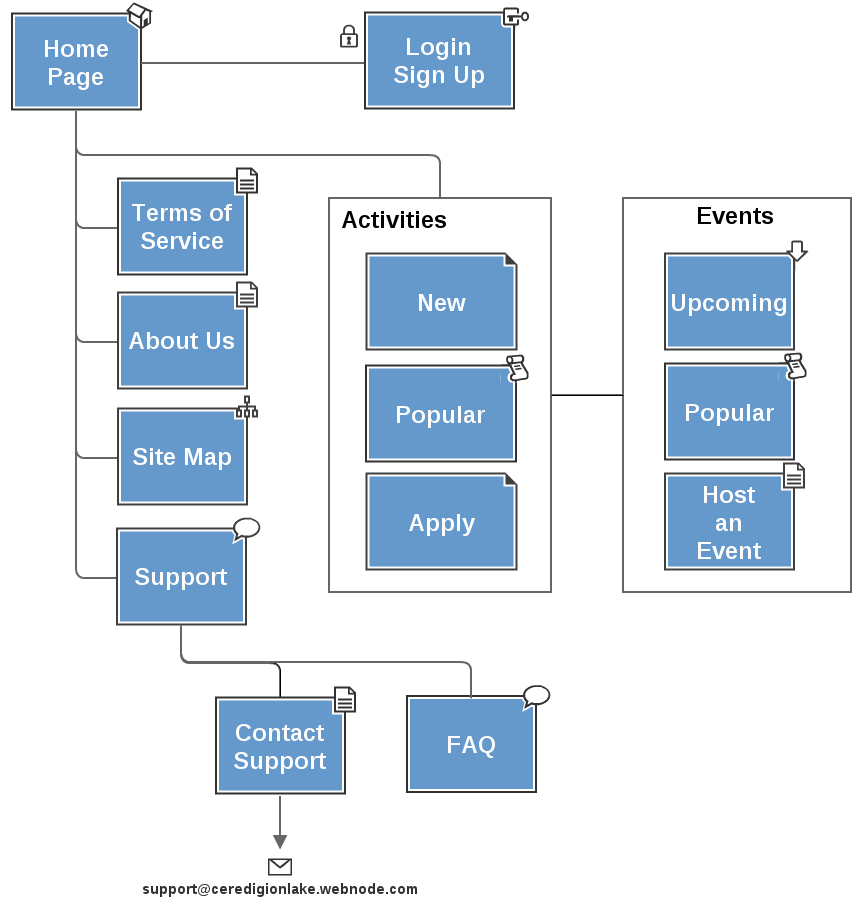
\includegraphics[width=5.0in] {IA.png}
%        \caption{IA Diagram}
%        \label{IA Diagram}
%\end{figure}

\section{Business Description}
Anti-Entropy is company specialising in mobile applications for back office sales systems.  The currently supported platforms are the iOS and Android operating systems.  The aim of this product is to give busineses a simple solution to managing information on customers, provided products and services.  This application may even replace dedicated terminals with a more convenient form factor, idealy installed on company supplied phones or tablets.
\\We also provide server hardware which hosts a central database the mobile software interacts with for its operations.  This can either be renting our hosting service or purchasing a dedicated server for installation on the customers premesis.
\\Along with the software and the server hardware we also offer support contract packages to help streamline the integration of our products into a customers business.

\section{Competitor Analysis}
The main competitors for this type of product would be similar products and the dedicated hardware versions as well as companies that offer similar back end sales management.
\\Companies that offer sich services are:
\begin{itemize}
\item ACT!
\\A CRM solution software package created by Sage.
\\This seems to be a Windows only solution with no Mac, Linux or mobile support apart from some standard calendar syncing features.
\\They also offer a support package at a cost.

\item Goldmine
\\It has a mobile version as well as a desktop version with integration into Microsoft Outlook.
\\The mobile version is only available on iOS and requires a windows server to host the service.
\\This solution also seems to have third party plugin support for a few additional features.

\item Maximizer
\\QIC Systems Ltd partners Maximizer CRM Which also has iCalendar integration as well as a web based access tot he system.
\\It has mobile versions as well including blackberry and windows mobile (not windows phone).

\end{itemize}



\section{Strengths}
We have solutions for the two main current mobile platforms as well as offering both hosted and dedicated database options.
\\Providing a personal service by having a friendly sales team who get to know each of our customers businesses directly and offer to meet on their own premesis.

\section{Weaknesses}
The costs of starting up and generating an initial income is the greatest weakness during the early stages of the business.
\\Competitors are already established and can already generate revenue to stay afloat.
\\\\The second weakness would be awareness, the competitors are already known or easily found.  Getting the brand out to potential customers and portraying our product as a quility brand.

\section{Opportunities}
The internet is a very cheap and effective medium for gaining awareness and for easy communication between us as a company and our customers.
\\Anti-Entropy will focus on good business to business relationships to try and establish brand loyalty and to help tailor our service to their individual needs.
\\A lot of these services are just a software package with optional support with no need to talk to a human being, just order the software and you are done, we offer a personal service to help integrate with existing businesses.

\section{Threats}
Already established products are much more likely to get the sales over a new unknown product.
\\If the venture is very successfull then there is the possibility of work overload where we may not be able to deliver all of the services promtly and to the standard of which the customer is expecting.

\section{Personnel}
\begin{itemize}
\item Managing Director
\\Will be responisble to the top level management of the business and making sure that all of the finances are managed appropriately.

\item Senior Developer
\\Responsible for the development team.  Should have a Computer Science or programming background.
\end{itemize}


\section{Marketing}


\end{document}
